\documentclass[10pt]{article}
\usepackage[margin=0.85in]{geometry}\usepackage[T1]{fontenc}\usepackage{lmodern,graphicx,booktabs,amsmath,xcolor,url}\usepackage[colorlinks=true,allcolors=blue]{hyperref}
\title{Acquiring Corrections Without Free Sibling Labels\\\large A bounded audit-and-transfer experiment on financial question answering}
\author{OverseeingManyLLMs research prototype}\date{12 September 2026}
\begin{document}\maketitle
\begin{abstract}
A correction obtained for one answer may help related work, but it may also damage an answer that was already correct. We implement a sequential protocol that chooses an answer to inspect, discloses only that question's annotation, and selectively regenerates related answers. Transfer outcomes become available to the learner only if their recipient is subsequently inspected. A frozen comparison uses 24 previously uninspected TAT-QA source contexts, 144 human-written questions, and two generated replicas. At two inspections, adaptive acquisition minus fixed acquisition changed official exact match by -2.08 percentage points, 95\% paired interval [-4.86, 0.35]. The method produced 16 helpful and 24 harmful regeneration events. This study does not establish a correctness advantage for adaptive acquisition over fixed acquisition with the same transfer mechanism. This result distinguishes a functioning feedback protocol from a demonstrated algorithmic advance.
\end{abstract}
\section{Question and protocol}
Users supervising several outputs may be able to reuse one correction, but shared source material does not establish shared error. Budgeted audit allocation and information acquisition are established ideas \cite{fleet,knowledge}. Agent Gym already provides scoped correction rules and collateral-match handling \cite{gym}. ExpeL retrieves reusable feedback \cite{expel}, while MACE adaptively selects peer interactions using quality rewards \cite{mace}. The present distinction is the feedback boundary. An uninspected recipient's private score cannot become an online reward.

For each question, the public state contains the source, generated answer and scale, inferred evidence references and acquired correction history. An inspection discloses only that question's answer, scale and derivation and directly replaces its answer. This is ideal annotation supervision. Siblings receive fallible generated continuations. A subsequent inspection may score that recipient's saved before/after states and update the model.

Let $e_j$ estimate error and let $f_r,h_r$ estimate repair and harm for an inferred relation. The recipient gain is
\[g(j,r)=e_j f_r-(1-e_j)h_r-0.01.\]
The last term is an assumed machine-cost preference. Acquisition ranks estimated local gain plus up to three positive recipient gains. Five-percent randomized selection is logged. Beta-smoothed development estimates initialize each episode; only purchased labels update them. Applicability and successful repair are not separately identifiable. This is an interpretable heuristic, without calibrated-confidence or regret guarantees.

At two inspections, the first disclosure can alter the next acquisition through error and co-error beliefs. A transition label acquired at the second inspection can affect its subsequent recipient choices, but not retrospectively select that inspection. A smaller three-inspection diagnostic tests a later acquisition. The format guard retains a previous answer when regeneration is malformed; it does not reject a valid wrong answer using private truth.

\section{Source, design and outcomes}
TAT-QA provides real report tables/prose and human-written benchmark questions \cite{tatqa}. Agent assignments, inspection episodes and supervision costs are constructed. We retain original question wording, disclose no sibling annotations and evaluate with the official EM/F1 code. Twelve training contexts support development. The final development pilot had 20/72 exact matches; 60 sibling transfers repaired nine errors and damaged six correct answers, compared with seven repairs and three harms from matched reattempts.

The held-out declaration was committed before generation. It fixes 24 public test-gold contexts, two replicas, seven methods and two inspections, plus small parameter-update and three-inspection diagnostics. Initial outputs are shared, while changed prompts receive actual GPU continuations. Seeds do not guarantee identical answers. Official scoring credits extracted answers, including 4 initial answers with invalid auxiliary or scale-schema fields. A separately labeled strict-schema rescore retains this ambiguity without changing the recorded online updates. The 24 source contexts are paired units; missing report identifiers prevent stronger report-level independence claims. No source was replaced after failure.

\begin{table}[ht]\centering\small
\begin{tabular}{lrrr}\toprule Method & Official EM & Sibling fixed/harmed & Recipient calls\\\midrule
Individual & 167/288 & 0/0 & 0 \\
Context memory & 165/288 & 24/26 & 432 \\
Source rule & 158/288 & 4/13 & 95 \\
Fixed acquisition & 162/288 & 15/20 & 186 \\
Adaptive & 156/288 & 14/21 & 189 \\
Reattempt & 164/288 & 1/4 & 95 \\
Risk-only individual & 170/288 & 0/0 & 0 \\
\bottomrule\end{tabular}
\caption{Two ideal inspections per context/replica, 288 answers per method. Sibling counts compare final never-inspected answers with their initial states. Inspected answers are replaced directly, and their correctness is not model repair.}\end{table}

The primary adaptive-minus-fixed comparison is -2.08 percentage points, 95\% paired interval [-4.86, 0.35], with wins/ties/losses 4/12/8. The practical comparison against risk-only individual inspection is -4.86 percentage points, 95\% paired interval [-9.72, 0.00]. Context-paired intervals use 2000 bootstrap resamples after averaging replicas. No noninferiority or equivalence claim follows from a wide interval containing zero. Additional comparisons are secondary.

\begin{figure}[ht]\centering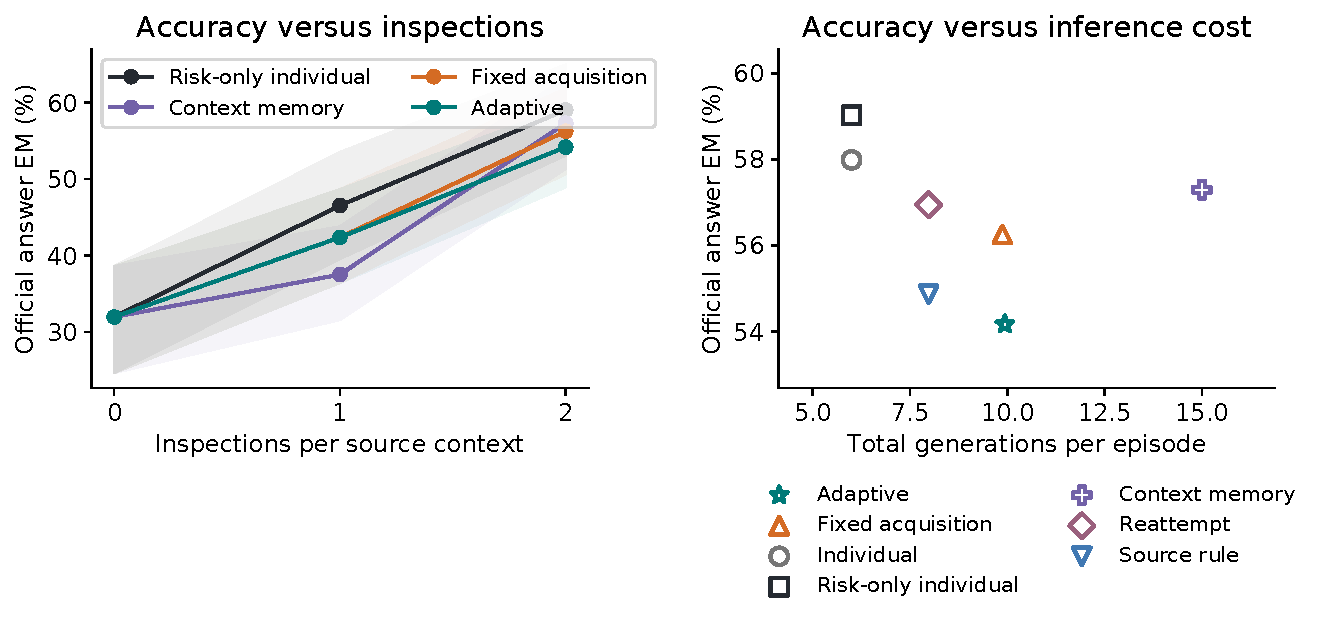
\includegraphics[width=\linewidth]{../../artifacts/adaptive_correction_transfer/figures/quality_cost.pdf}
\caption{Generated answers and ideal annotation feedback on held-out financial contexts. Bands are descriptive context-bootstrap intervals. Machine generations are distinct from human effort. Full policy tables accompany the figure.}\end{figure}

\section{Transfer, adaptation and alternatives}
Adaptive and fixed acquisition chose different inspection sequences in 39/48 episodes. The source-rule versus reattempt contrast is -2.08 percentage points, 95\% paired interval [-5.90, 1.74]. This comparison keeps inspected questions, feedback format, recipient sets and sampling settings matched. It tests correction information beyond the value of an extra generation. Actual identical requests also varied in 23 request groups, so action differences and generation variability must be distinguished.

\begin{figure}[ht]\centering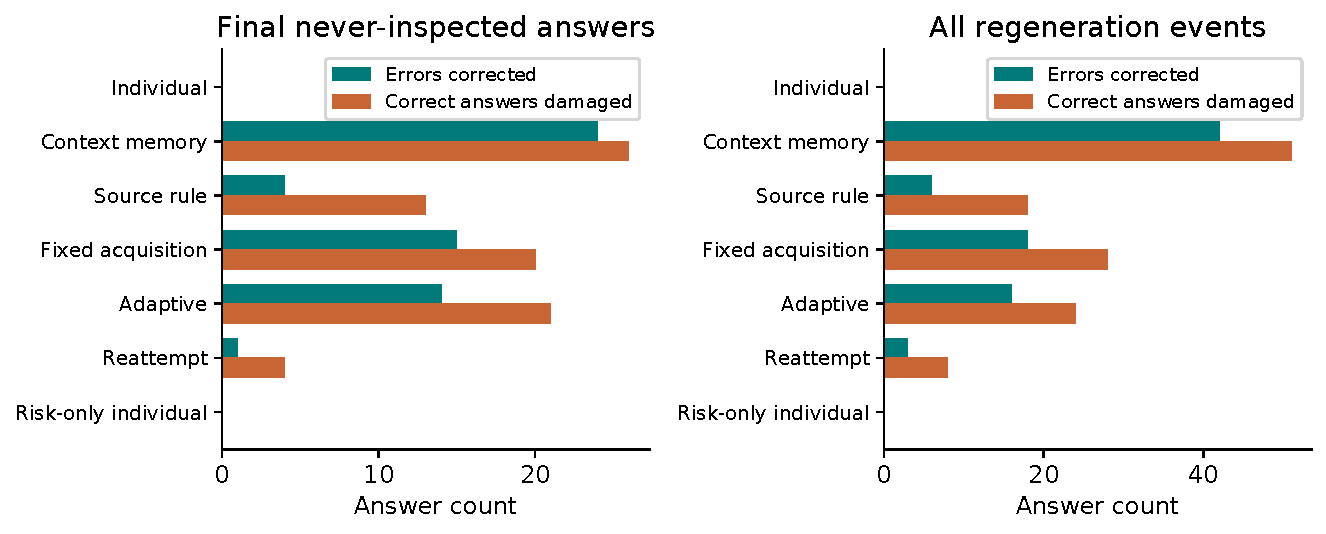
\includegraphics[width=\linewidth]{../../artifacts/adaptive_correction_transfer/figures/transfer_and_harm.pdf}
\caption{Helpful and harmful generated changes are retained. Final never-inspected output counts and repeated regeneration-event counts are different quantities. Private labels are used only for this offline analysis.}\end{figure}

The final adaptive outputs contain 14 newly correct and 21 newly wrong never-inspected answers. Sparse development relations and limited generated evidence localization constrain recipient selection. Fixed acquisition corrected 80 currently wrong inspected answers, versus 72 for adaptive acquisition. Regeneration had net effects of -10 and -8, respectively, accounting for the final six-answer difference. Disabling parameter updates changed no inspections, recipient membership or correctness in twelve diagnostic episodes; one recipient execution order changed. At three inspections, adaptive minus fixed EM was -8.33 percentage points, with a descriptive paired interval [-14.58, -2.08] across eight contexts. The same source can support a monetary amount and a scale-invariant ratio, so copying a scale or inferred explanation may be inappropriate. A verified answer alone need not reveal an error's root cause.

\begin{figure}[ht]\centering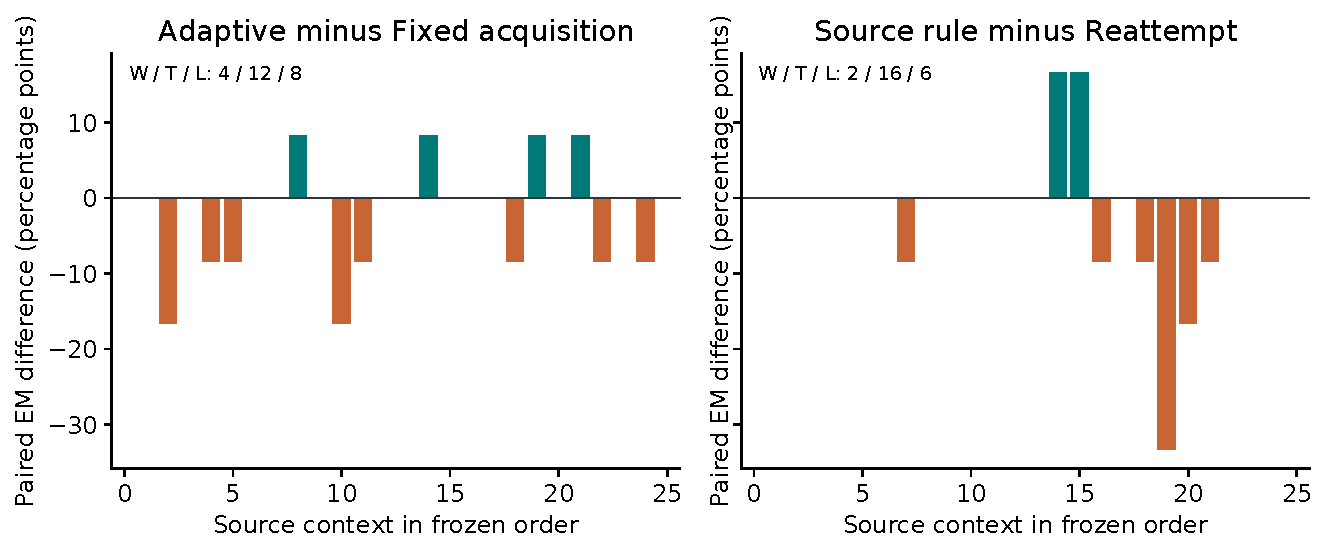
\includegraphics[width=\linewidth]{../../artifacts/adaptive_correction_transfer/figures/paired_sources.pdf}
\caption{Each bar is a source-context mean across two generated replicas. Positive values favor the first policy. Neither agent roles nor repeated policy runs increase the number of source units.}\end{figure}

Eight synthetic mechanisms use 32 fixed seeds each and scripted response processes. They retain independent errors, correlated errors, misleading similarity, partial applicability, scale exceptions and ineffective repairs. Helpful and unfavorable regimes are both present. These fixtures establish protocol boundaries, not natural prevalence or a rescue for the empirical comparison.

\section{Practical system and conclusion}
The local Decision desk shows the next inspection, shared evidence, the question-specific disclosure, inferred recipients and their actual before/after outputs. Future feedback and uninspected correctness remain hidden. Replay reconstructs all 364 completed traces using only recorded disclosures. Sixteen focused tests, 51 historical checks and nine browser checks validate the implementation boundary. Scripted interaction logs are not participant observations.

This study does not establish a correctness advantage for adaptive acquisition over fixed acquisition with the same transfer mechanism. A practical improvement over risk-only individual correction is not established. The supported contribution is an executable acquisition-and-transfer protocol and a controlled measurement of helpful and harmful reuse under selectively observed feedback. It is not evidence that shared memory, adaptive selection or multiple agents are intrinsically superior. Individual QA competence and recipient applicability must improve before additional acquisition complexity can be justified. Human correction effort, fallible human review, independently identified reports and single-agent architectural comparisons remain unmeasured.

The stage used 2083 scheduled calls and 2058 generation attempts on an existing Qwen2.5-7B BF16 GPU service, with no CPU model offload. All failures and earlier development versions are retained. Reproduction, full diagnostics, source attribution and resource records are in \texttt{research/adaptive\_correction\_transfer/}. The historical submission remains unchanged.
\bibliographystyle{plainurl}\bibliography{references}
\end{document}
